\documentclass[conference]{IEEEtran}
\IEEEoverridecommandlockouts

\usepackage{amsmath,amssymb,amsfonts}
\usepackage{graphicx}
\usepackage{textcomp}
\usepackage{xcolor}
\usepackage{booktabs}
\usepackage{tabularx}
\usepackage{hyperref}
\usepackage{float}
\usepackage{placeins}
\usepackage{balance}

\hypersetup{
    hidelinks
}

\begin{document}

\title{Numerical and Machine Learning Methods for Solving Apoptosis Ordinary Differential Equations}

\author{
\IEEEauthorblockN{
\begin{tabular}{c}
Dana Hamed, Habiba Ibrahim, Rana Hesham, Menna Ashraf, Nour Ahmed \\
David Bahaa, Ebrahim Nasser, Filopatir Emad, Yahya Ismail \\
Youssef El Roby, Youssef Hisham
\end{tabular}
}
\IEEEauthorblockA{
Department of Systems and Biomedical Engineering, Faculty of Engineering, Cairo University\\
Giza, Egypt
}
}

\maketitle

\begin{abstract}
This paper presents a numerical and learning-based study of apoptosis, a regulated programmed cell death process commonly modeled using ordinary differential equations (ODEs) in biomedical systems biology \cite{kutumova2025,burt2022}. The apoptosis pathway is represented using a six-variable nonlinear ODE system involving HIF-1$\alpha$, oxygen/reactive oxygen species (ROS), p300 co-activator, p53 tumor suppressor, caspase, and potassium-related signaling based on Schiesser's biomedical ODE model \cite{schiesser2014}. Two classical numerical methods, Forward Euler and fourth-order Runge-Kutta (RK4), are implemented and compared. In addition, a Physics-Informed Neural Network (PINN) is developed to approximate the continuous solution while enforcing the ODE physics and initial conditions. Three cases are tested: a base case, an all-zero initial condition case, and a time-varying coupling case with $\alpha_{12}(t)=0.10e^{-0.05t}$. The results show that RK4 is more accurate and stable than Euler, while the PINN closely matches the RK4 ground truth with low relative L2 errors.
\end{abstract}

\begin{IEEEkeywords}
Apoptosis, Ordinary Differential Equations, Forward Euler, RK4, Physics-Informed Neural Networks, Biomedical Simulation.
\end{IEEEkeywords}

\section{Introduction}
Apoptosis is a regulated form of programmed cell death that plays an essential role in tissue homeostasis, embryonic development, immune regulation, and elimination of damaged or abnormal cells. Dysregulation of apoptosis is associated with cancer, autoimmune disease, and degenerative disorders. Since apoptosis depends on interacting biochemical regulators, mathematical modeling provides a useful way to study its dynamic behavior over time.

This project solves a six-variable apoptosis ODE model using both classical numerical methods and a machine-learning-based method. The objective is to compare Forward Euler, RK4, and a Physics-Informed Neural Network (PINN) in terms of accuracy, stability, and ability to reproduce apoptosis dynamics. The numerical methods provide direct time-stepping solutions, while the PINN provides a continuous differentiable approximation constrained by the same governing biological equations.

\section{Literature Review}

Mathematical modeling and machine learning are increasingly integrated to understand regulated cell death pathways.

\subsection{Mathematical Modeling of Cell Death}
Kutumova et al. \cite{kutumova2025} highlighted that dynamic apoptosis networks are effectively captured using ODE systems involving critical molecular regulators like p53 and caspases.

\subsection{Data-Driven Apoptosis Regulation}
Burt et al. \cite{burt2022} demonstrated that accurate survival modeling requires tracking direct caspase regulation, which strongly supports its central inclusion in our ODE system.

\subsection{Deep Learning and Cell Death Prediction}
Schorpp et al. \cite{schorpp2023} introduced CellDeathPred, proving the utility of deep learning in cell death analysis. This growing trend justifies our implementation of Physics-Informed Neural Networks (PINNs) as a continuous surrogate solver.

\subsection{Detection Methods and Tissue-Level Effects}
Biological biomarkers like caspases ground these models in biological reality \cite{kari2022}. Furthermore, recent studies show that apoptosis profoundly alters tissue rigidity and fluidization \cite{softmatter2022,prl2024}, guiding future multiscale extensions of our ODE model.

\begin{table}[htbp]
\caption{Summary of Reviewed Literature}
\label{tab:lit_review}
\centering
\small
\begin{tabularx}{\linewidth}{l X}
\toprule
\textbf{Reference} & \textbf{Relevance to This Work} \\
\midrule
\cite{kutumova2025} & Supports ODE-based modeling of regulated cell death pathways. \\
\cite{burt2022} & Shows the importance of caspase regulation in apoptosis survival models. \\
\cite{schorpp2023} & Demonstrates the value of deep learning in apoptosis-related analysis. \\
\cite{kari2022} & Explains apoptosis biomarkers and detection methods. \\
\cite{softmatter2022,prl2024} & Support future tissue-scale extension of apoptosis modeling. \\
\bottomrule
\end{tabularx}
\end{table}

\section{Methodology}

\subsection{Apoptosis ODE Model}
The model used in this project is a six-variable nonlinear ODE system based on Schiesser's apoptosis biochemical cascade \cite{schiesser2014}. The state vector is:
\begin{equation}
\mathbf{y}=[y_{hif},y_{o2},y_{p300},y_{p53},y_{casp},y_{kp}]^T.
\end{equation}

The variables represent HIF-1$\alpha$, oxygen/ROS, p300, p53, caspase, and potassium-related signaling. The implemented system is:
\begin{align}
\dot{y}_{hif}  &= a_{hif} - a_3\, y_{o2}\, y_{hif} - a_4\, y_{hif}\, y_{p300} - a_7\, y_{p53}\, y_{hif} \\
\dot{y}_{o2}   &= a_{o2}  - a_3\, y_{o2}\, y_{hif} + a_4\, y_{hif}\, y_{p300} - a_{11}\, y_{o2} \\
\dot{y}_{p300} &= a_8     - a_4\, y_{hif}\, y_{p300} - a_5\, y_{p300}\, y_{p53} \\
\dot{y}_{p53}  &= a_{p53} - a_5\, y_{p300}\, y_{p53} - a_9\, y_{p53} \\
\dot{y}_{casp} &= a_{12}(t) + a_9\, y_{p53} - a_{13}\, y_{casp} \\
\dot{y}_{kp}   &= -a_{10}\, y_{casp}\, y_{kp} + a_{11}\, y_{o2} - a_{14}\, y_{kp}
\end{align}

The parameter values from Table~3.3 of Schiesser \cite{schiesser2014} are:

\begin{table}[h]
\centering
\caption{Model Parameters (Schiesser Table 3.3)}
\begin{tabular}{llll}
\hline
Parameter & Value & Parameter & Value \\
\hline
$a_{hif}$ & 1.52  & $a_8$    & 0.06  \\
$a_{o2}$  & 1.80  & $a_9$    & 0.10  \\
$a_{p53}$ & 0.05  & $a_{10}$ & 0.70  \\
$a_3$     & 0.90  & $a_{11}$ & 0.20  \\
$a_4$     & 0.20  & $a_{12}$ & 0.10  \\
$a_5$     & 0.001 & $a_{13}$ & 0.10  \\
$a_7$     & 0.70  & $a_{14}$ & 0.05  \\
\hline
\end{tabular}
\end{table}

\begin{figure}[htbp]
\centering

\includegraphics[width=0.95\linewidth]{fig_apoptosis_6vars.png}
\caption{Dynamic evolution of the six apoptosis ODE state variables under Case 1 conditions.}
\label{fig:ode_dynamics}
\end{figure}

\subsection{Numerical Methods}
The first numerical method was Forward Euler:
\begin{equation}
\mathbf{y}_{n+1}=\mathbf{y}_n+h\mathbf{f}(t_n,\mathbf{y}_n),
\end{equation}
which is simple but first-order accurate. The second method was RK4:
\begin{equation}
\mathbf{y}_{n+1}=\mathbf{y}_n+\frac{h}{6}(k_1+2k_2+2k_3+k_4),
\end{equation}
where $k_1,k_2,k_3,k_4$ are the four RK4 slopes. RK4 is fourth-order accurate and was also used as the ground truth reference for evaluating the PINN.

\subsection{Physics-Informed Neural Network}
The PINN approximates the continuous solution as:
\begin{equation}
\hat{\mathbf{y}}(t;\theta)=[\hat{y}_{hif},\hat{y}_{o2},\hat{y}_{p300},\hat{y}_{p53},\hat{y}_{casp},\hat{y}_{kp}]^T.
\end{equation}

The network uses one input neuron for time, six output neurons for the state variables, six hidden layers, 128 neurons per hidden layer, and Tanh activations. Case 1 uses a Softplus final activation to prevent negative concentrations. The loss function combines the ODE residual and the initial condition loss:
\begin{equation}
\mathcal{L}_{total}=w_{ode}\mathcal{L}_{ode}+w_{ic}\mathcal{L}_{ic}.
\end{equation}

The ODE residual is:
\begin{equation}
\mathcal{L}_{ode}=\frac{1}{N}\sum_{j=1}^{N}\left\|
\frac{d\hat{\mathbf{y}}(t_j)}{dt}-\mathbf{f}(t_j,\hat{\mathbf{y}}(t_j))
\right\|^2.
\end{equation}
The PINN was trained using Adam followed by L-BFGS optimization, with $w_{ic}=1000$ to strongly enforce the initial condition.

\subsection{Experimental Cases}
Three cases were evaluated. Case 1 used $\mathbf{y}(0)=[1,0,0,0,0,0]$ and constant $\alpha_{12}=0.10$. Case 2 used $\mathbf{y}(0)=[0,0,0,0,0,0]$ and constant $\alpha_{12}=0.10$. Case 3 used the same initial condition as Case 1 but with time-varying coupling:
\begin{equation}
\alpha_{12}(t)=0.10e^{-0.1t}.
\end{equation}

\section{Results and Discussion}

\subsection{Numerical Solver Results}
The numerical simulations showed that the apoptosis ODE system rapidly moves from its initial transient response toward a stable equilibrium region. In Case 1, HIF-1$\alpha$ decreased from its initial value while oxygen/ROS, p300, caspase, and potassium-related variables increased toward steady-state levels. Case 2 started from all-zero initial conditions, but the production terms drove the system toward nearly the same equilibrium region as Case 1, showing that the constant-coupling model is asymptotically stable for the tested conditions.

At $h=0.1$, Forward Euler produced an RMSE of $0.000644$, while RK4 produced an RMSE of $0.0000150$. Although Euler is faster per step, it accumulates larger error because it uses only the derivative at the beginning of each step. RK4 is more computationally expensive per step, but its higher-order slope averaging provides much better accuracy and stability.

\begin{figure}[htbp]
\centering
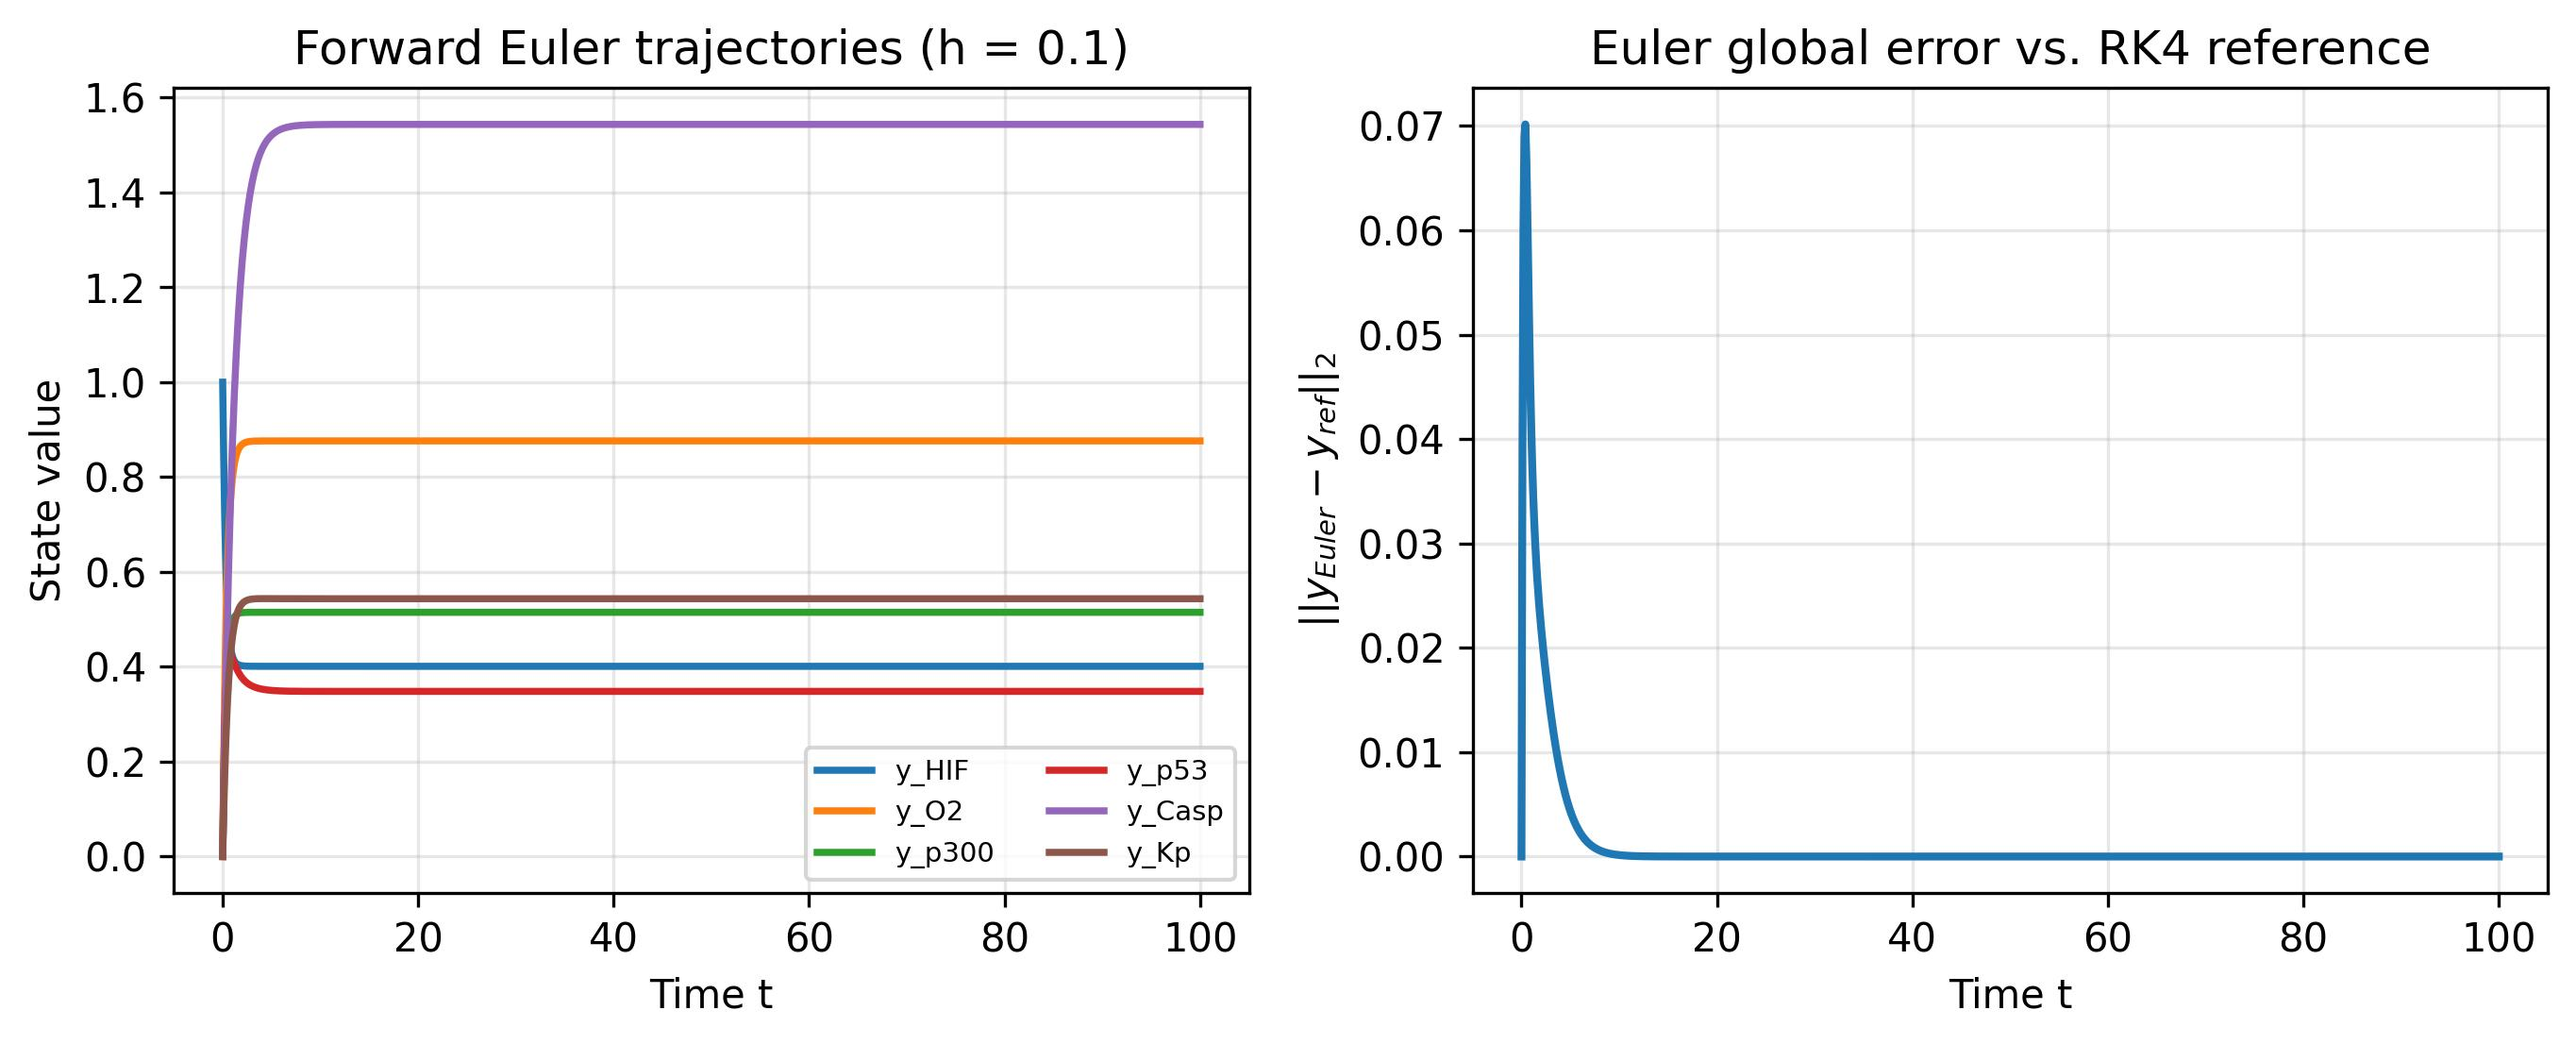
\includegraphics[width=0.95\linewidth]{euler.jpeg}
\caption{Forward Euler simulation and error behavior at step size $h=0.1$.}
\label{fig:euler}
\end{figure}

\begin{figure}[htbp]
\centering
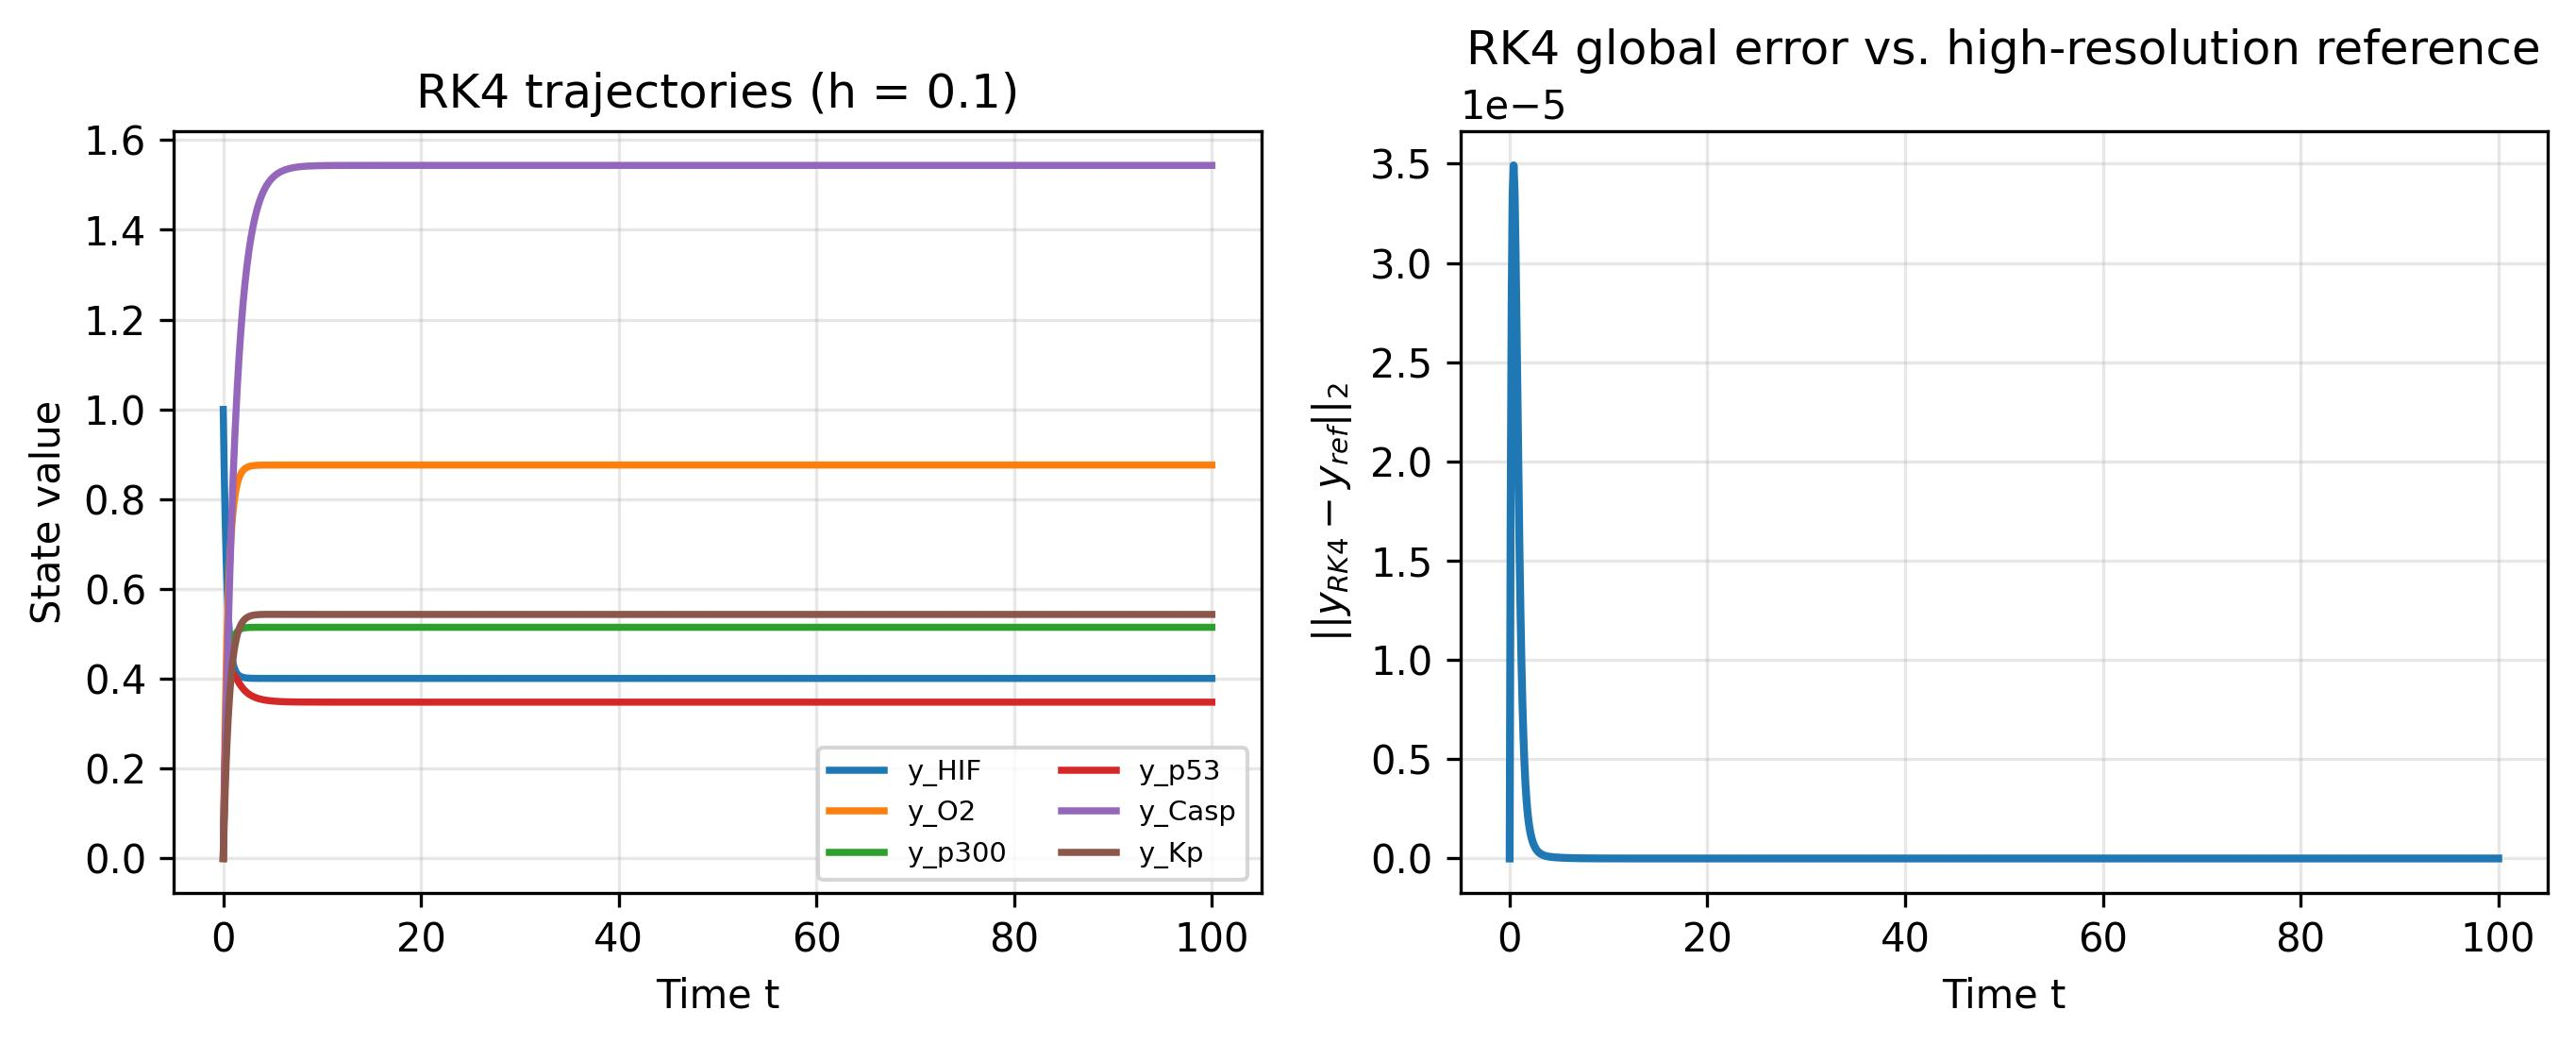
\includegraphics[width=0.95\linewidth]{rk4.jpeg}
\caption{RK4 simulation and error behavior at step size $h=0.1$.}
\label{fig:rk4}
\end{figure}

Under Case 3, the exponentially decaying coupling coefficient introduced non-stationary behavior. Euler showed larger accumulated error under this dynamic setting, while RK4 maintained stronger stability. This confirms that RK4 is more robust when model parameters vary with time.

\begin{figure}[htbp]
\centering

\includegraphics[width=0.95\linewidth]{fig_apoptosis_a12_variation.png}
\caption{Effect of exponentially decaying coupling $\alpha_{12}(t)=0.10e^{-0.05t}$ on apoptosis ODE trajectories.}
\label{fig:a12}
\end{figure}

\subsection{PINN Results}
The PINN results were compared with RK4 ground truth using relative L2 error. The PINN achieved low errors for all variables and cases, with the smallest error for caspase in Case 2 ($0.037\%$) and the largest for HIF-1$\alpha$ in Case 1 ($0.218\%$). These results demonstrate that the PINN successfully learned a continuous approximation of the apoptosis trajectories while satisfying the physical ODE constraints.

\begin{table}[htbp]
\centering
\caption{PINN Relative L2 Errors Against RK4 Ground Truth}
\label{tab:pinn_errors}
\small
\begin{tabular}{lccc}
\toprule
\textbf{Variable} & \textbf{Case 1} & \textbf{Case 2} & \textbf{Case 3} \\
\midrule
$y_{hif}$  & 0.218\% & 0.115\% & 0.119\% \\
$y_{o2}$   & 0.086\% & 0.048\% & 0.064\% \\
$y_{p300}$ & 0.116\% & 0.091\% & 0.102\% \\
$y_{p53}$  & 0.106\% & 0.125\% & 0.109\% \\
$y_{casp}$ & 0.064\% & 0.037\% & 0.097\% \\
$y_{kp}$   & 0.107\% & 0.067\% & 0.085\% \\
\bottomrule
\end{tabular}
\end{table}

Unlike Euler and RK4, which compute discrete time-step values, the PINN learns a differentiable function that can be evaluated at any time point inside the training interval. This makes it useful as a continuous surrogate model for interpolation, visualization, and future parameter estimation. However, the PINN requires an upfront training phase, so RK4 remains simpler and more efficient for a single direct simulation.

\begin{figure}[htbp]
\centering
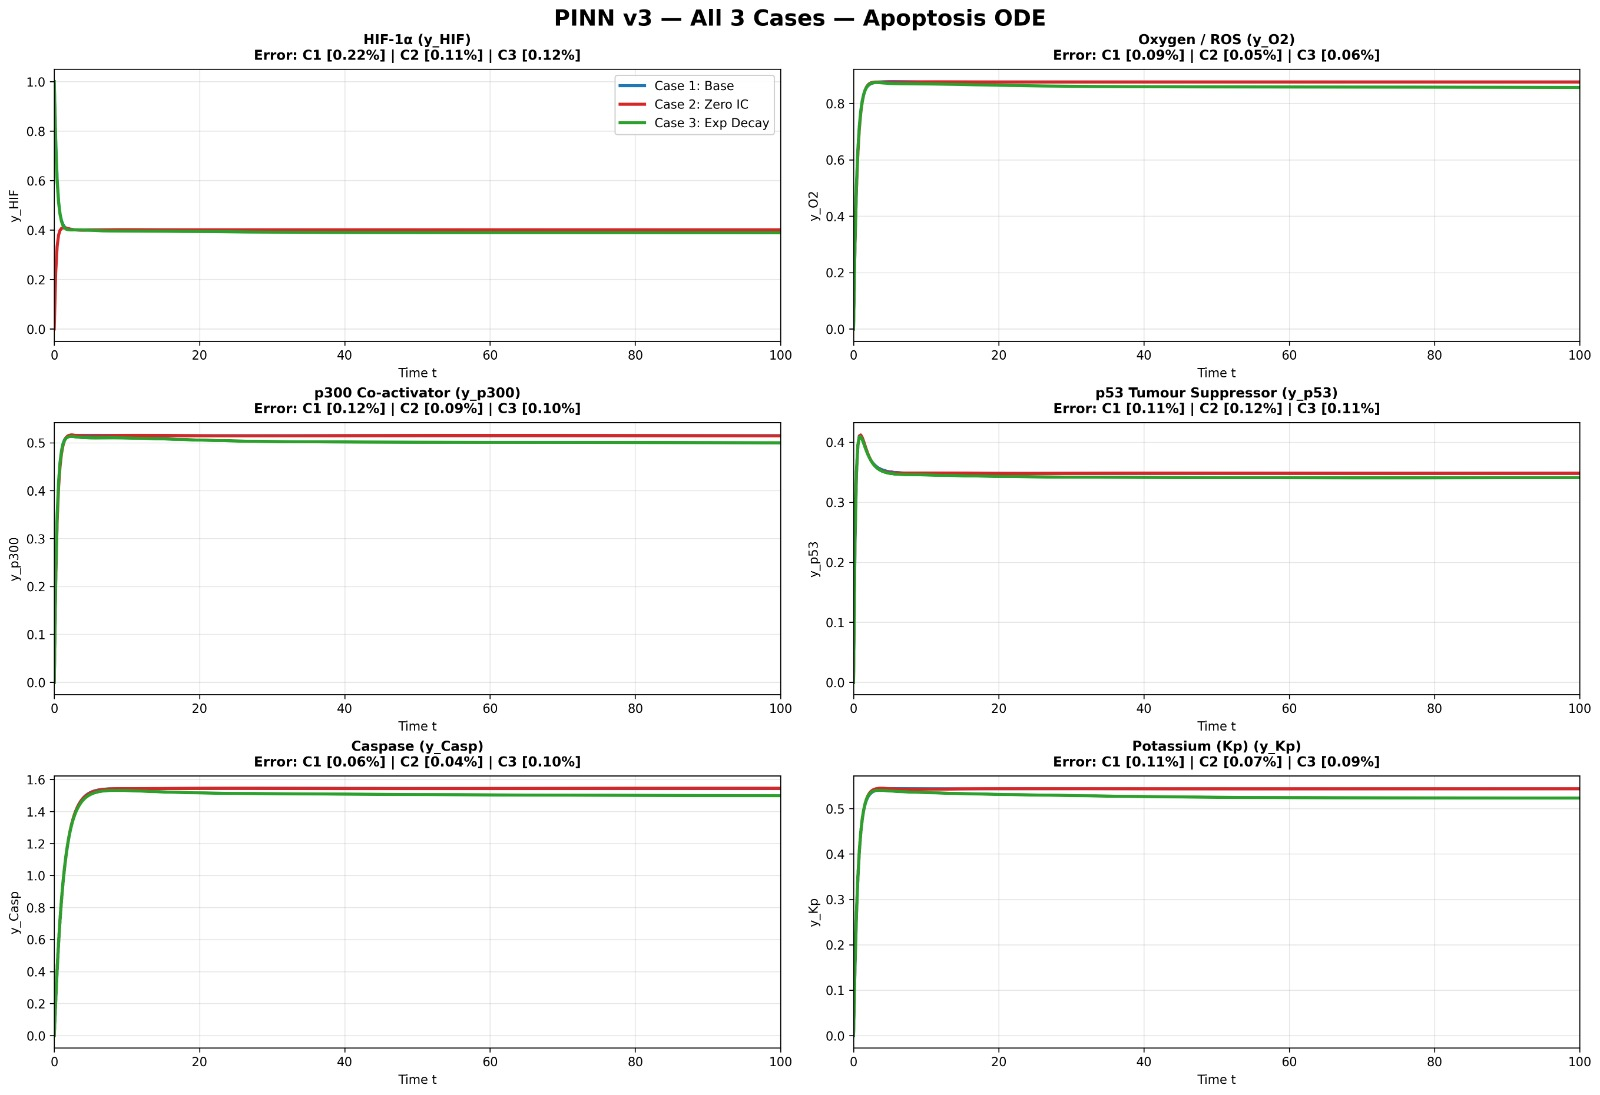
\includegraphics[width=0.95\linewidth]{pinn_all_cases_evaluated.png}
\caption{PINN predictions for all three apoptosis cases across the six state variables.}
\label{fig:pinn_all_cases}
\end{figure}

For Case 1, the PINN followed the RK4 reference solution closely after the initial transient. For Case 2, the model successfully learned the system behavior from an all-zero initial state. For Case 3, the PINN captured the effect of the decaying coupling coefficient and remained close to the RK4 reference trajectory.

\begin{figure}[htbp]
\centering
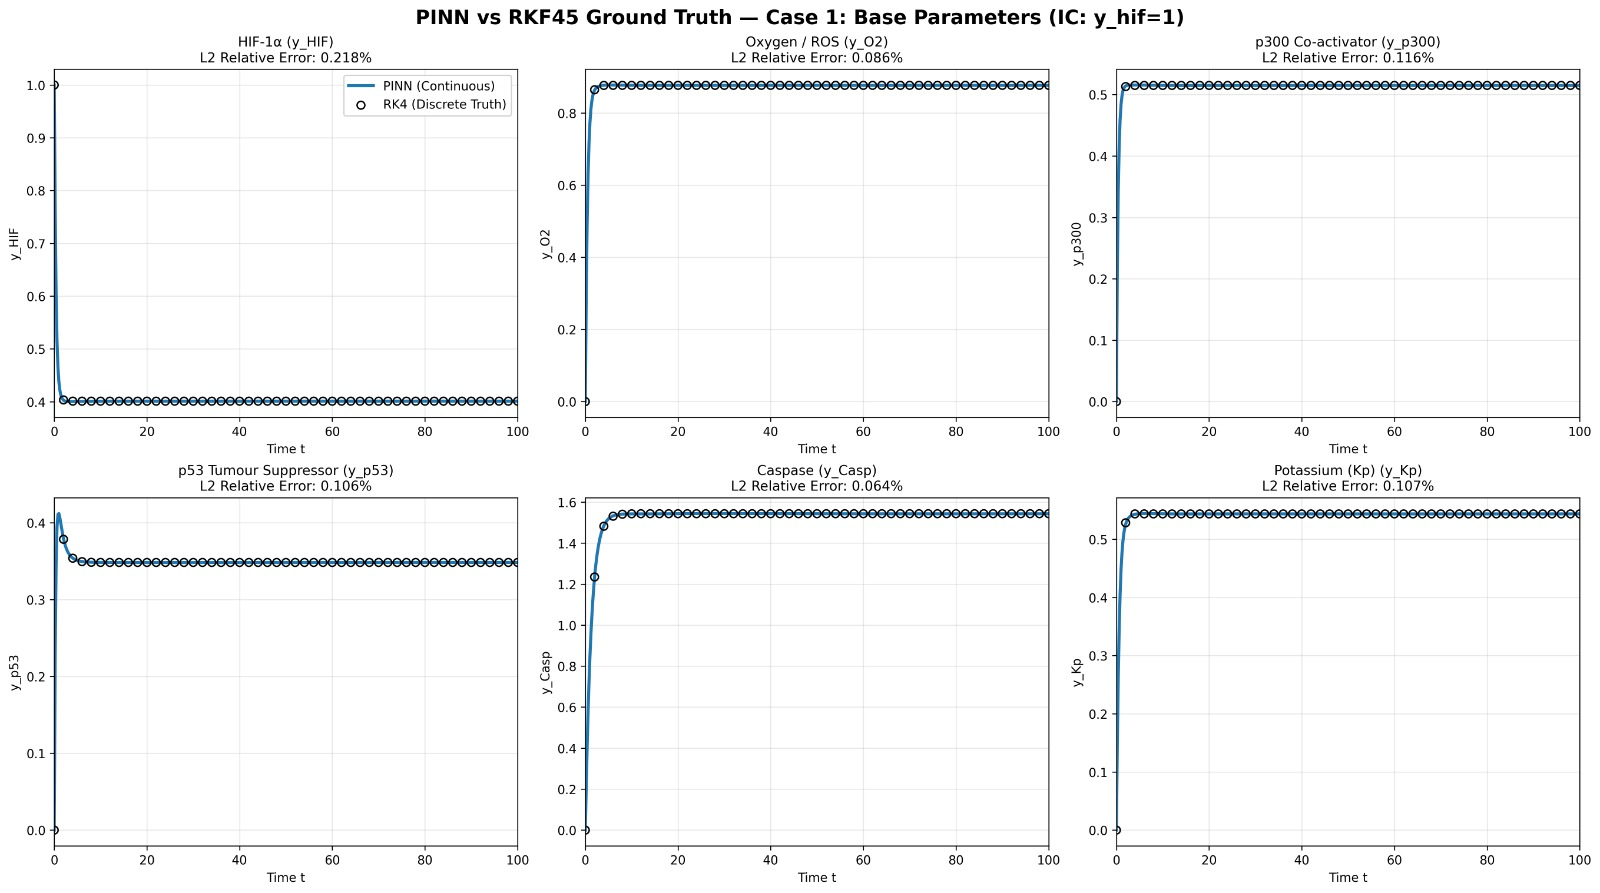
\includegraphics[width=0.95\linewidth]{pinn_case1_individual.png}
\caption{Case 1 PINN prediction compared with RK4 ground truth.}
\label{fig:pinn_case1}
\end{figure}

\begin{figure}[H]
\centering
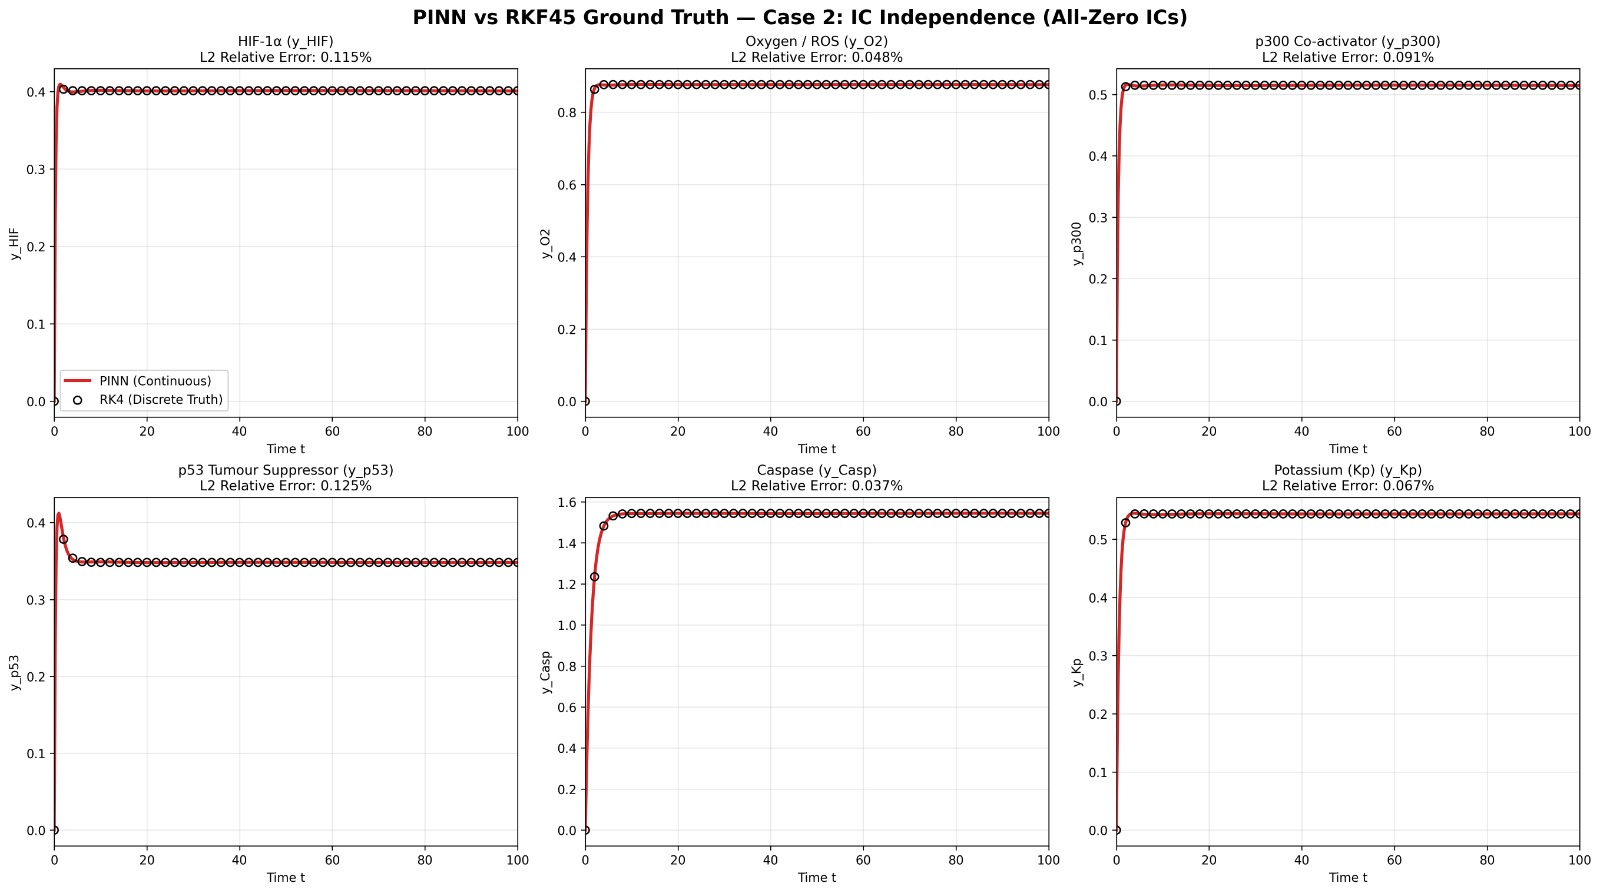
\includegraphics[width=0.95\linewidth]{pinn_case2_individual.png}
\caption{Case 2 PINN prediction compared with RK4 ground truth under all-zero initial conditions.}
\label{fig:pinn_case2}
\end{figure}

\begin{figure}[H]
\centering
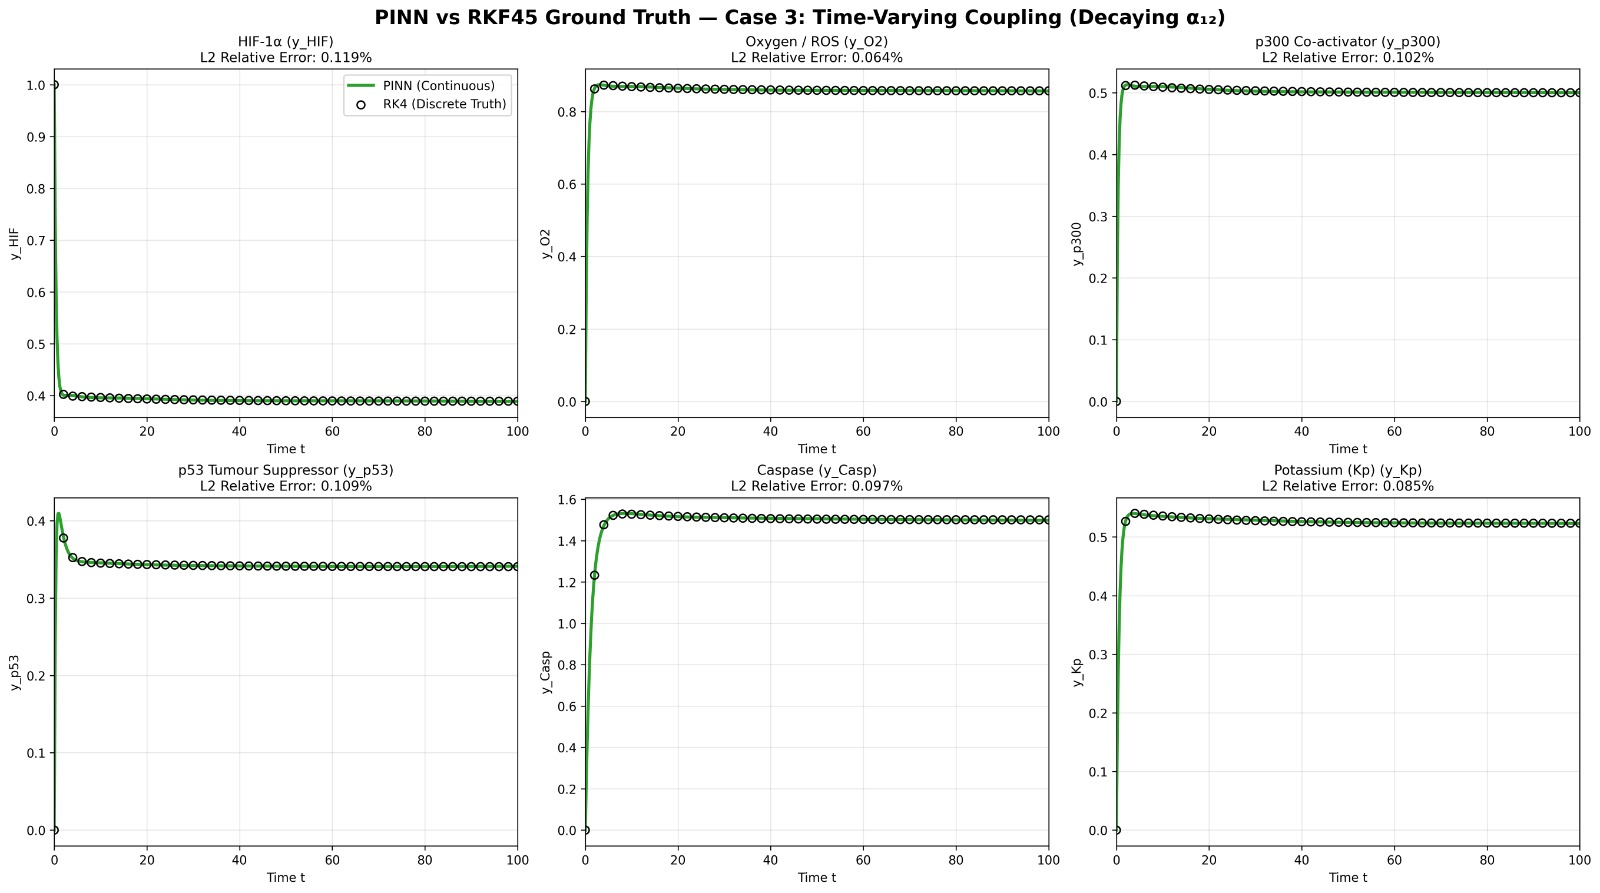
\includegraphics[width=0.95\linewidth]{pinn_case3_individual.png}
\caption{Case 3 PINN prediction compared with RK4 ground truth under time-varying coupling.}
\label{fig:pinn_case3}
\end{figure}

\FloatBarrier
\section{Conclusion}
This project implemented and compared numerical and machine-learning methods for solving a six-variable apoptosis ODE system. Forward Euler, RK4, and PINN approaches were evaluated under base, zero-initial-condition, and time-varying-coupling cases. The results showed that RK4 is more accurate and robust than Forward Euler, especially when the coupling parameter changes over time. The PINN successfully approximated the continuous apoptosis trajectories and achieved low relative L2 errors compared with RK4 ground truth. Therefore, RK4 is the most reliable classical solver for direct simulation, while PINNs provide a promising continuous surrogate modeling approach for future biomedical simulation and parameter-estimation tasks.

\section{Future Work}
Future work can extend the current model by including more detailed apoptosis regulators such as BAX, Bcl-2, mitochondrial cytochrome c release, and pathway crosstalk with necroptosis or pyroptosis. The model can also be coupled with tissue-level simulations to study how apoptosis affects tissue rigidity and organization. In addition, PINNs can be used for inverse modeling to estimate unknown biological parameters from experimental data.



\begin{thebibliography}{00}

\bibitem{kutumova2025}
E. Kutumova, I. Akberdin, I. Lavrik, and F. Kolpakov, ``Mathematical Modeling of Cell Death and Survival: Toward an Integrated Computational Framework for Multi-Decision Regulatory Dynamics,'' \textit{Cells}, vol. 14, no. 22, p. 1792, 2025.

\bibitem{burt2022}
P. Burt, R. Cornelis, G. Gei{\ss}ler, S. Hahne, A. Radbruch, H.-D. Chang, and K. Thurley, ``Data-Driven Mathematical Model of Apoptosis Regulation in Memory Plasma Cells,'' \textit{Cells}, vol. 11, no. 9, p. 1547, 2022.

\bibitem{schorpp2023}
K. Schorpp, A. Bessadok, A. Biibosunov, I. Rothenaigner, S. Strasser, T. Peng, and K. Hadian, ``CellDeathPred: a deep learning framework for ferroptosis and apoptosis prediction based on cell painting,'' \textit{Cell Death Discovery}, vol. 9, p. 277, 2023.

\bibitem{kari2022}
S. Kari, K. Subramanian, I. A. Altomonte, A. Murugesan, O. Yli-Harja, and M. Kandhavelu, ``Programmed cell death detection methods: a systematic review and a categorical comparison,'' \textit{Apoptosis}, vol. 27, pp. 482--508, 2022.

\bibitem{softmatter2022}
G. A. Reddy and P. Katira, ``Differences in Cell Death and Division Rules Can Alter Tissue Rigidity and Fluidization,'' \textit{Soft Matter}, 2022, doi: 10.1039/D2SM00174H.

\bibitem{prl2024}
Y. Tang, S. Chen, M. J. Bowick, and D. Bi, ``Cell Division and Motility Enable Hexatic Order in Biological Tissues,'' \textit{Physical Review Letters}, 2024.

\bibitem{schiesser2014}
W. E. Schiesser, \textit{Differential Equation Analysis in Biomedical Science and Engineering: Ordinary Differential Equations with R}. John Wiley \& Sons, 2014.

\end{thebibliography}

\end{document}